\section{Pregunta N$^{\circ}$12\qquad León Alonzo Terrones Caccha}

\begin{frame}
    
Dado el problema de valor inicial

              \begin{equation}
                  \begin{cases}
                      y^\prime =\dfrac{3x-2y}{x}
                       & \\
                      t\in [0,0.2]
                       & y\left(0\right)=1
                  \end{cases},
              \end{equation}
tiene solución $y(t)=1-\log(1-et)$. Aplicar el método de Adams de tercer paso.
              

    \begin{solution}

    \begin{figure}
        \centering
        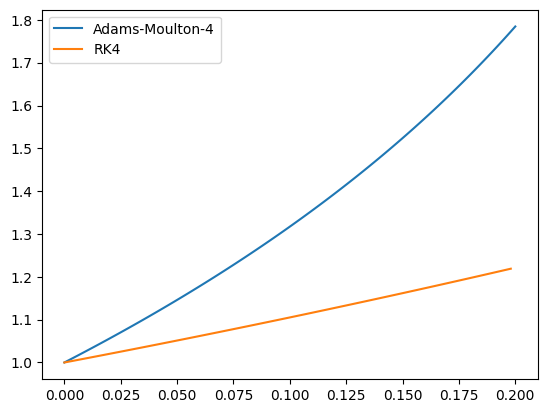
\includegraphics[width=8cm]{p12-Comparar-results.png}
        %\caption{Caption}
        \label{fig:enter-label}
    \end{figure}
    \end{solution}
\end{frame}
\begin{frame}{}
    \begin{figure}
        \centering
        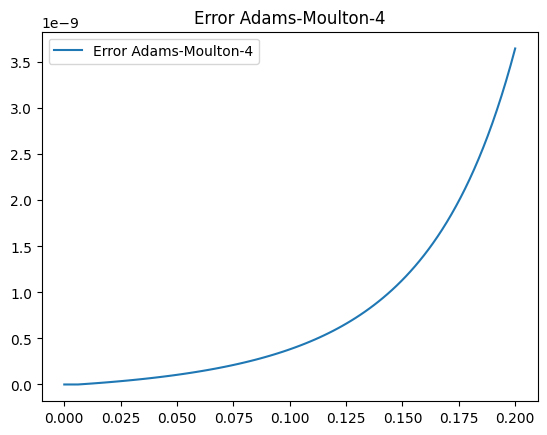
\includegraphics[width=8cm]{p12-Error-AM.png}
        %\caption{Caption}
        \label{fig:enter-label}
    \end{figure}
\end{frame}

\begin{frame}{}
    \begin{figure}
        \centering
        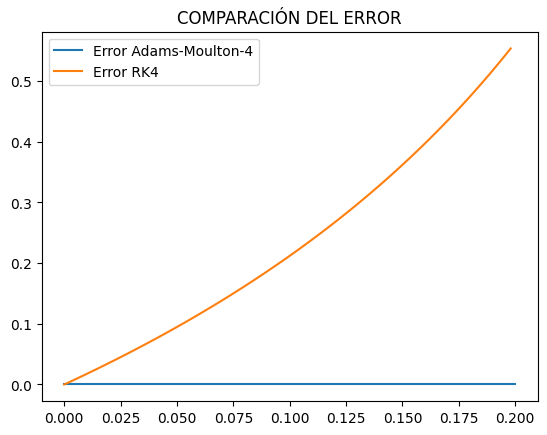
\includegraphics[width=8cm]{p12-Comp-error.png}
        %\caption{Caption}
        \label{fig:enter-label}
    \end{figure}
\end{frame}